\section{The Cleaning Service}
\label{sec:cleaning}

This section presents an automated cleaning \emph{service}, which focuses on identifying problems that can be cleaned (based on the report of the quality assessment service described in Deliverable 5.2~\cite{diachron-d5.2}) and automatically cleaning an RDF dataset by removing all problematic triples, as well as an interactive cleaning \emph{application}, which supports a human user in resolving more complex cleaning problems.

The general functionality as well as architecture of the cleaning module, which have been introduced in Deliverable 3.1~\cite{d3.1}, remains unchanged.
The cleaning process is composed of the three following steps:
\begin{enumerate}
	\item\label{it:assess} Identifying quality problems in a dataset (carried out by the implementation described in Deliverable 5.2~\cite{diachron-d5.2})
	\item\label{it:suggest} Suggesting transformations to fix these problems
	\item\label{it:apply} Applying these transformations to the dataset
\end{enumerate}

The cleaning \emph{service} takes care of steps (\ref{it:assess}) and (\ref{it:suggest}), and (\ref{it:apply}), where the ``transformation rule'' is simplified to ``delete all triples affected by quality problems''.
In contrast to repairing, which applies unambiguously specified rules to data that violate logical constraints, data cleaning cannot be performed \emph{fully} automatically, because the correction of errors and inconsistencies requires user involvement as well as detailed knowledge of the data. 
Therefore, to provide full support for cleaning, we have additionally developed an interactive (review and approval of cleaning suggestions by the user) and iterative (sequential processing of the identified problems) cleaning \emph{application}.

Designing and implementing the cleaning process raises three main difficulties.
First, since human resources are very expensive it is necessary to automate as much work as possible and give the user maximal support so that a well-founded decision can be taken. 
Second, because of the iterative nature of the cleaning process it is essential to be able to set up the cleaning process according to the user's needs. 
Third, allowing the user to work interactively – in the cleaning application – requires the availability of a user friendly interface.

The Diachron cleaning service and application address these requirements in the following ways:

\begin{enumerate}
\item The cleaning service is designed in a way to provide as much automated operation as possible. For that the identification of quality problems and generation of cleaning suggestions are done automatically in the background.
We maintain concrete user advices and data transformation rules in an extensible ontology.
\item The interface both of the service and of the application enables the user (human or machine) to specify quality metrics he is interested in (see more details in section~\ref{sec:serviceDescription}).
\item  We implemented the cleaning application as an extension to the well-known cleaning tool OpenRefine\footnote{\url{http://openrefine.org/}}. This enables to use a wide range of functionalities provided in OpenRefine, such as defining and applying transformation on the data in a spreadsheet like interface (see Figure \ref{fig:spreadsheet}).
Transformation effects are immediately displayed on the screen and each single transformation can be undone.  
\end{enumerate}


\subsection{Service Description}
\label{sec:serviceDescription}

The main components of the cleaning service and the cleaning application were defined according to the three steps of the cleaning process, presented above, namely: i) a component for quality problems identification, ii) a component for generating cleaning suggestions, and iii) a component for applying cleaning rules.

The general description of the cleaning service and application, as well as architecture design, have been introduced in Deliverable 3.1~\cite{d3.1}.
Hereafter we present a detailed description of the particular service components as well as design decisions and implementation details that have been made.
Since the quality assessment service already exists in Diachron (see Deliverable 5.2 \cite{diachron-d5.1} for more details), the cleaning service and application were designed to operate on its output.
In order to provide the user with an interactive application for data cleaning that enables to define and apply cleaning operations in a spreadsheet-like interface we decided to implement the cleaning application as an extension of the well-known data cleaning tool OpenRefine.

\textbf{OpenRefine} (formerly Google Refine) is a powerful tool for working with data containing inconsistences and invalidities. 
It serves a wide range of functionalities for: detecting and fixing inconsistencies; transforming data from one structure or format to another; looking up further information from web services; and linking it to databases like Freebase.
OpenRefine  is a stand-alone desktop application. 
It supports ``expressions'' to transform existing data or to create new data based on existing data.
OpenRefine supports several languages for writing expressions. It has its own native language called OpenRefine Expression Language (GREL), but other languages such as Jython\footnote{\url{https://github.com/OpenRefine/OpenRefine/wiki/Jython}} are also supported. Detailed information of how to work with OpenRefine is presented in~\cite{verborgh_packt_2013}.

Combining the Diachron quality assessment framework and the OpenRefine cleaning framework has two advantages: the former can automatically identify inconsistences and anomalies in data, while the latter serves a wide range of functionalities designed for interactive data cleaning.

Both the data cleaning service and the data cleaning application accept as input a possibly erroneous and inconsistent data set and output a cleaned data set.
The complete transformation from the input data into to the output view is decomposed into three steps, each of which corresponds to the specific service component, described below in more detail.
First, we present the complete cleaning workflow using the Diachron quality extension for OpenRefine.

\subsubsection{Cleaning Workflow}
\label{sec:workflow}

Figure~\ref{fig:workflow} shows the whole workflow of the cleaning process.
Hereafter we explain it step by step, illustrated by screenshots of the cleaning application.
Typical usage of the cleaning service, whose API is presented separately in section~\ref{sec:service-API}, follows a similar but simplified workflow.
For now, we take the perspective of the user controlling the whole workflow from inside OpenRefine: the user loads a dataset, has its quality assessed, and then cleans.
For subsequent stages of code integration, we are aiming at enabling external applications to embed our cleaning application into more complex workflows.
See, e.g., Deliverable 5.2~\cite[section~4.3]{diachron-d5.2} for a full quality assessment workflow, one of whose steps is cleaning.

\begin{figure}[ht!]
\centering
\includegraphics[page=14,trim=1.0cm 1.0cm 1.0cm 1.0cm,clip,width=\textwidth]{figures/cleaning.pdf}
\caption{Cleaning process workflow}
\label{fig:workflow}
\end{figure}

The user starts cleaning by uploading his data and creating a new project. OpenRefine supports several data formats, including RDF and Turtle. The uploaded data set will be displayed to the user; now the cleaning process can begin.

Clicking on the `Diachron Quality' extension button and then selecting `Identify Quality Problems' tab  (Figure~\ref{fig:tab}), the user launches the interface where he can specify  the quality metrics of his interest (Figure~\ref{fig:interface}). If he only wants to work on specific metric  dimensions or even single metrics, he can click the corresponding checkboxes. 
\begin{figure}[ht!]
\centering
\includegraphics[width=.6\textwidth]{figures/extension.png}
\caption{The Diachron Quality extension  menu to OpenRefine}
\label{fig:tab}
\end{figure}
\begin{figure}[ht!]
\centering
\includegraphics[width=.75\textwidth]{figures/metricSelection.png}
\caption{Selecting quality metrics for which problems should be identified}
\label{fig:interface}
\end{figure}

Once the selection of quality metrics has been confirmed by clicking the `OK' button, the quality assessment service will be invoked to perform quality assessment and return a quality report.
The quality report is an input for the `cleaning suggestion generation' component.
Cleaning suggestions are generated based on the quality report ontology, presented in more detail in section~\ref{sec:cleaningSuggestions}. Each quality problem in the ontology is assigned with an appropriate cleaning suggestion and, if available, an cleaning rule (see section~\ref{sec:cleaningSuggestions} for more details). 
In preparation for the next cleaning step, the original data set is displayed in a spreadsheet view with the following columns: Subject, Predicate, Object, Quality Problem, Problem Description, Cleaning suggestion and Cleaning Rule (Figure~\ref{fig:spreadsheet}).

\begin{figure}[ht!]
\centering
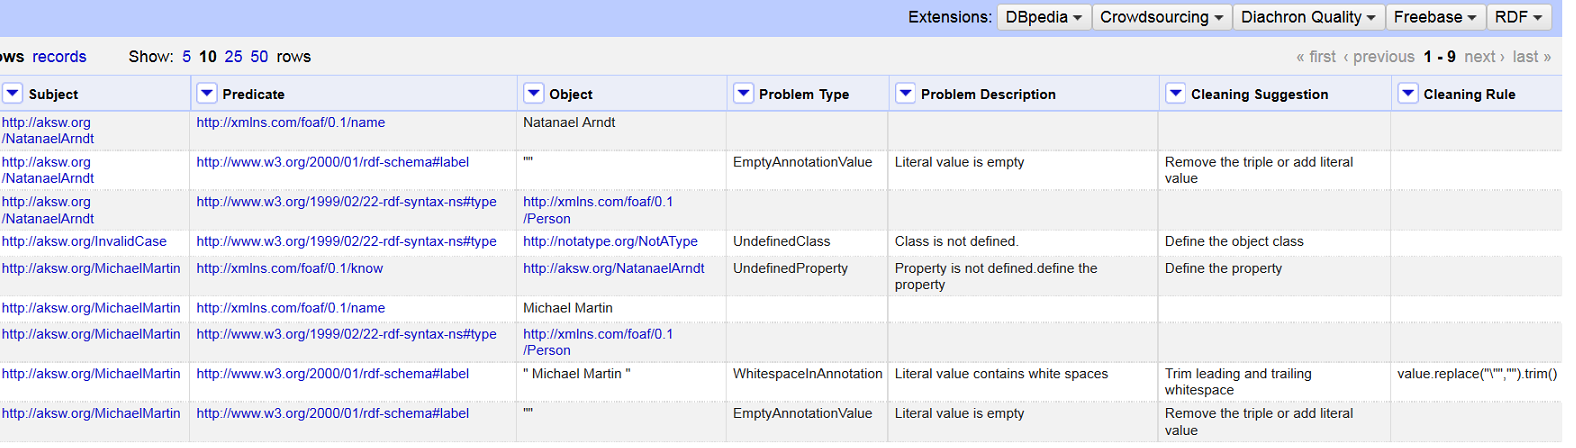
\includegraphics[width=\textwidth]{figures/spreadsheet.png}
\caption{Dataset with the corresponding quality problems and cleaning suggestions.}
\label{fig:spreadsheet}
\end{figure}
This view enables the user to work separately on each single triple component, e.g.\ to apply a transformation only to the predicate column or to perform changes in the object column.
OpenRefine supports faceted browsing as a mechanism for filtering down to just a subset of rows to be transformed.
Faceting enables to filter all the triples affected by a particular quality problem, and to apply a proposed data transformation rule to relevant triples only.
After defining a text facet over the possible values of the Quality Problem column, the left panel will display all identified quality problems with the number of their occurrences (Figure~\ref{fig:facets}).
Sorting them the user can sequentially clean the dataset w.r.t.\ these problems, starting with the most frequent one. 

\begin{figure}[ht!]
\centering
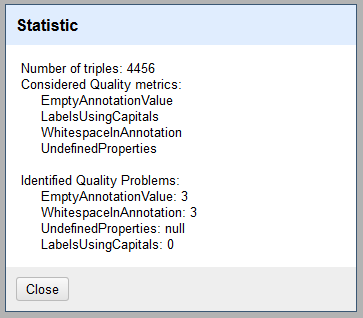
\includegraphics[width=.99\textwidth]{figures/statistics.png}
\caption{Data filtered by a particular quality problem. Quality problems, sorted by frequency, are displayed  in the left panel}
\label{fig:facets}
\end{figure}

Unfortunately, it is not always possible to define an appropriate data transformation as GREL rule. 
For some problems, such as `EmptyAnnotationValue', the user has to fill in the value manually, or he should remove the corresponding triple.
The proposed rule can be applied in the corresponding view (see Figure \ref{fig:transformation}). After putting the proposed expression into the expression field, the user can directly see the effect of the targeted transformation. 
\begin{figure}[ht!]
\centering
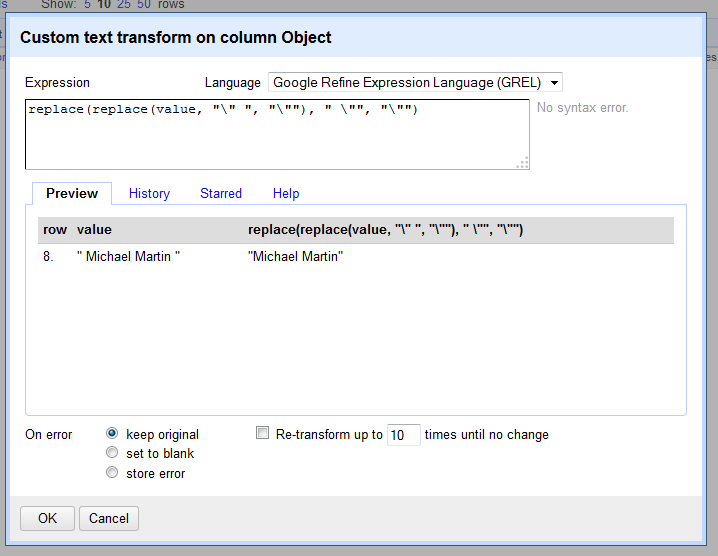
\includegraphics[width=.75\textwidth]{figures/transformation.png}
\caption{Data transformation view.}
\label{fig:transformation}
\end{figure}
After cleaning, the user can download the cleaned data set in the original format.


\subsubsection{Quality Problem Identification}

As mentioned above, the core of the Quality Problem identification component is the Diachron quality assessment service, which was introduced in Deliverable 5.1~\cite{diachron-d5.1} and is described in detail in Deliverable 5.2~\cite{diachron-d5.2}.
The quality assessment framework enables to reflect different aspects of data quality, with regard to a wide range of quality metrics.
In parallel to \emph{computing} any quality metric, it collects those triples that violate the quality criteria defined by the particular metric. 
Two different outputs are provided: the quality metadata, i.e.\ an RDF representation of metric values, and the quality report, which is composed of identified quality problems.
The quality report (QR) is represented in terms of the QR ontology, which we developed for this purpose, and which is described in Deliverable 5.2~\cite[section 2.1.1]{diachron-d5.2}.

An ontology represents the concepts and their relations that are relevant for a given domain \cite{Wang05anontology-based}. It consists of a representational vocabulary with precise definitions of the meanings of the terms in the vocabulary plus a set of axioms. The QR ontology was designed to specify the concepts related to quality problems and possible solution for them. 
 
Figure~\ref{fig:ontology1} shows the structure of the quality report vocabulary.
The \texttt{Quality report} is \texttt{computedOn}  a \texttt{Resource} and \texttt{contains}  a set of \texttt{Quality problems}. 

\begin{figure}[ht!]
\centering
\includegraphics[page=5,trim=0.2cm 8.0cm 1.0cm 6.0cm,clip,width=\textwidth]{figures/cleaning.pdf}
\caption{General structure of the Quality Report ontology}
\label{fig:ontology1}
\end{figure}

With respect to Deliverable 3.1~\cite{d3.1} the QR ontology was extended to support cleaning issues as described in the next section.

\subsubsection{Generation of Cleaning Suggestions}
\label{sec:cleaningSuggestions}

Figure~\ref{fig:ontology2} presents the extended structure of the \texttt{QualityProblem} class. 
A \texttt{QualityProblem} is \texttt{describedBy} the corresponding \texttt{Metric} and \texttt{affects} an RDF triple, which we reify for the purpose of referring to it. 
A problem's \texttt{problemDescription} property aims to provide the user with a brief and clear description of the problem.
The \texttt{cleaningSuggestion} property contains a general natural language recommendation how to solve the identified problem, while the optional \texttt{cleaningRule} property contains a cleaning rule.
The latter property has language-specific subproperties, such as \texttt{grelCleaningRule} for cleaning rules expressed in GREL.

The quality report contains a set of quality problems that are associated with the affected triples.
As soon as we are able to precisely refer to a quality problem by URI, it is straightforward to provide the user with an appropriate cleaning suggestion and with additional information (such as an exact description description of the problem) to help the user understand. 
The property \texttt{describedBy} is not bijective, as one quality metric may correspond to one or more quality problems. 
Consider, for example, the \texttt{MisusedOwlDatatypeOrObjectProperty} metric.
From a high-level quality assessment perspective it is not important to separately count datatype properties and object properties that were misused; any triple with any such misuse just counts as one ``bad'' triple.
However, it does play an important role from the cleaning  perspective, as the cleaning service and application aim at giving the user precise feedback.
We therefore relate to the two quality problems \texttt{MisusedDatatypeProperty} and \texttt{MisusedObjectProperty}, each of which has a different cleaning suggestion (see Table~\ref{tab:qualityProblems}). 
Some quality problems require additional properties in order to precisely specify the problem.
Figure \ref{fig:ontology3} shows an example for such kind of quality problems. 
In order to provide the user with an appropriate cleaning rule for \texttt{IncompatibleDatatypeRangeProblem} we need to memorize which datatype is required.  This is realized using the \texttt{qr:expectedDatatype} property.

The descriptions of concrete quality problems are available as a linked dataset at \url{http://purl.org/eis/vocab/qprob}.

\begin{figure}[ht!]
\centering
\includegraphics[page=3,trim=0.2cm 8.5cm 1.0cm 8.0cm,clip,width=\textwidth]{figures/cleaning.pdf}
\caption{Quality Problem Class of the QR vocabulary.}
\label{fig:ontology2}
\end{figure}


\begin{figure}[ht!]
\centering
\includegraphics[page=4,trim=0.2cm 9.5cm 0.2cm 6.5cm,clip,width=\textwidth]{figures/cleaning.pdf}\caption{Quality problem representation  in the QR Vocabulary.}
\label{fig:ontology3}
\end{figure}
\label{sub:generation}

\lstinputlisting[caption={An example of a quality problem},label=lst:quality_pr]{figures/ontology.trig}


\subsubsection{Transformation Engine}
The user performs data transformation by direct manipulation on the OpenRefine spreadsheet interface. 
He first chooses an appropriate column and selects rows affected by a particular quality problem using facets. 
Working step by step on the quality problems identified, the user can undo particular transformations if they do not have the expected effect.
This positively affects the accuracy of cleaning results.
Having performed all necessary transformations on the data, the user can export the cleaned data to their original RDF format.
\begin{table}[t]
\caption{Quality Problems}
\label{tab:qualityProblems}
\begin{center}
\begin{tabular}{p{.13\textwidth}p{.36\textwidth}p{.3\textwidth}p{.2\textwidth}}                                                                                                                                           \\ 
\bf{Dimension} & \bf{Quality Problem}                    & \bf{Problem Description}                                             & \bf{Cleaning suggestion}                                                              \\ \hline \\
Availability   & \texttt{SPARQLAccessibility}            & SPARQL Endpoint can not be accessed                                  & Check the SPARQL Endpoint URI or remove the triple                                    \\
               & \texttt{RDFDumpAcccessibility}          & RDF dump is not available                                            & Check the path to RDF dump or remove the triple                                       \\
               & \texttt{NotValidURI}                    & URI is not valid or link is broken                                   &                                                                                       \\
               & \texttt{UnstructuredData}               & Dead link                                                            & Check the way the vocabulary is published or use a different one                      \\
               % & \texttt{NoDereferencedBackLinks}        & The backlink is not dereferenced                                     &                                                                                       \\
%              & dereferencability of forward-links      & detection of no dereferenced forward-links                           & Problem report                                                                        \\ \hline \\
Accuracy       & \texttt{MalformedDatatypeLiteral}       & Literal value is not consistent with its data type                   & Convert literal to expected datatype                                                  \\
	       & \texttt{expectedDatatype rdfs:Datatype} &                                                                      &                                                                                       \\
	       & \texttt{IncompatibleDatatypeRange}      & Literal value is not consistent with property range                  & Convert literal to expected datatype                                                  \\
	       & \texttt{expectedDatatype rdfs:Datatype} &                                                                      &                                                                                       \\
	       & \texttt{HomogeneousDatatypes}           & Property has literals of different datatypes as its objects          & Convert literals to unique datatype                                                   \\
Consistency    & \texttt{MisplacedClass}                 & Instance of \texttt{rdfs:Class} used in property position            & Use instance of \texttt{rdf:Property}                                                 \\
               & \texttt{MisplacedProperty}              & Instance of \texttt{rdf:Property} used in object position            & Use instance of \texttt{rdfs:Class}                                                   \\
               & \texttt{MisusedOwlDatatypeProperty}     & \texttt{owl:DatatypeProperty} is used with \texttt{rdfs:Resource}    & Use class of \texttt{owl:ObjectProperty} or change object to \texttt{rdfs:Literal}    \\
               & \texttt{MisusedOwlObjectProperty}       & \texttt{owl:ObjectProperty} is used with \texttt{rdfs:Literal}       & Use class of \texttt{owl:DatatypeProperty} or change object to \texttt{rdfs:Resource} \\
Representation & \texttt{WhitespaceInAnnotation}         & Literal value contains leading or trailing whitespaces               & Trim leading and trailing whitespace                                                  \\
               & \texttt{EmptyAnnotationValue}           & Literal value is empty                                               & Remove the triple or add literal value                                                \\
               & \texttt{LabelsUsingCapitals}            & Literal uses a bad style of capitalization                           & Change the capitalization of the literal                                              \\
               & \texttt{BlankNodeObject}                & Object is a blank node (i.e.\ neither a literal nor a resource having a URI) &                                                                                       \\
               & \texttt{BlankNodeSubject}               & Subject is a blank node           &                                                                                       \\
               & \texttt{OntologyHijacking}              & The triple redefines an element that already exists in an external vocabulary                              & Remove the triple or change it.
\end{tabular}
\end{center}
\end{table}

\subsection{Technical Documentation}


\subsubsection{Prerequisites}

\textbf{Apache Jena}
\label{sec:Jena}
Apache Jena
%\footnote{\url{https://jena.apache.org}} 
is an open source Semantic Web framework for Java. 
It provides a programmatic environment for RDF, RDFS and OWL, SPARQL and includes a rule-based inference engine. 
It provides an API to extract data from and write to RDF graphs. The graphs are represented as an abstract ``model''.  A model can be populated with data from files, databases, URLs or a combination of these. A model can be queried using SPARQL.

\textbf{Ontologies}
The \textbf{daQ}, \textbf{DQM}, and \textbf{QR} ontologies developed in the context of the Diachron project\footnote{\url{http://github.com/diachron/quality/}} are required to understand the quality report created by the quality assesment component and then to produce cleaning suggestion for the corresponding problems.

\textbf{OpenRefine} 
OpenRefine\footnote{\url{http://openrefine.org/}} is a desktop application for data cleaning, which provides the foundation for the cleaning application.
It is intended to be installed and run on the user's local machine, but has a web-based user interface.
Unlike most other desktop applications, it runs as a small web server on the local machine.
The user has to point the web browser at that web server in order to use OpenRefine. 

\subsubsection{Deployment Process}

Similarly to deploying the repairing service, as explained in section~\ref{sec:repair-deploy}, deploying the cleaning service involves the deployment of a WAR file, and defining the following parameters in a \textit{properties} file:

\begin{description}
\item[Quality\_Assessment\_Service:] The URL of the quality assessment web service required (see section~\ref{sec:cleaning-require}).
\end{description}

The cleaning application is implemented as an extension to OpenRefine and provided as a ZIP file.
Installing it requires extracting that ZIP file to the \textit{extensions} folder of the OpenRefine workspace and restarting OpenRefine.

\subsubsection{Required Web Service Interfaces}
\label{sec:cleaning-require}

The cleaning service requires the quality assessment service explained in Deliverable 5.2~\cite[section~2.4]{diachron-d5.2}.

\subsubsection{Exposed Web Service Interfaces}
\label{sec:service-API}

Deliverable 6.1 was missing a description of the RESTful API of the cleaning service, but explained the general design of these APIs for the Diachron services~\cite{diachron-d6.1}.
The cleaning service API is similar to the API of the quality assessment service described in Deliverable 5.2~\cite{diachron-d5.2}.

The cleaning service provides the two methods \texttt{/diachron/get\_cleaning\_suggestions} and \texttt{/diachron/clean}, of which we give a precise description below.
The typical usage of the cleaning service follows the workflow outlined for the cleaning application in figure~\ref{fig:workflow}:
In the input to the \texttt{get\_cleaning\_suggestions} method, the client specifies the dataset and the metrics w.r.t.\ which the dataset should be cleaned; the method returns a set of cleaning suggestions.
In the input to the \texttt{clean} method, the client one more specifies a set of metrics.
The dataset is then cleaned by applying the rule ``delete every triple that is affected by a quality problem w.r.t.\ to at least one of the metrics specified''.
This results in a cleaned dataset.
Optionally, the \texttt{clean} method returns – similarly to the \texttt{repair} method introduced in section – a list of all triples that were removed by cleaning.

\begin{table}[h]
\captionsetup{justification=raggedright,singlelinecheck=false}
\caption{Cleaning Methods}
\label{tbl:valid_meth}
\begin{tabular}{|p{5cm}|p{10cm}|}
\hline
\multicolumn{2}{|l|}{\textbf{Methods}} \\ \hline

\textbf{Modifier and Type} & 
\textbf{Method and Description} \\ \hline

\texttt{javax.ws.rs.core.Response} & 
\texttt{getCleaningSuggestionsJSON(java.lang.String inputMessage)}:
\textbf{POST} method which returns a set of cleaning suggestions. \\ \hline

\texttt{javax.ws.rs.core.Response} & 
\texttt{cleanJSON(java.lang.String inputMessage)}:
\textbf{POST} method which cleans a dataset (similar to the repair method described in section~\ref{sec:repair-expose}). \\ \hline

\hline
\end{tabular}
\end{table}

\subparagraph{Method Details}

\begin{description}

\item{\textbf{getCleaningSuggestionsJSON}:} \textbf{POST} method which returns a set of cleaning suggestions.

\textbf{URL (partial):} \url{/diachron/get_cleaning_suggestions} 

\textbf{Parameters}: 
\begin{itemize}
\item \texttt{inputMessage}: A JSON-encoded string which has the following form: \\
\{ \\
\hspace*{0.5 cm}"Dataset" : "Dataset1", \\
\hspace*{0.5 cm}"MetricsConfiguration" : "MetricsConfiguration", \\ 
\} \\
where : 
\begin{description}
\item[Dataset:] The URI of a DIACHRON entity to be validated. 
\item[MetricsConfiguration:] a list of quality metrics w.r.t.\ which cleaning suggestions should be generated.  The format of this list is defined by the quality assessment service and explained in \cite[section~2.4]{diachron-d5.2}. 
\end{description}

\end{itemize}
\textbf{Returns}: A Response instance which has a JSON-encoded entity content depending on the input parameter of the method. We discriminate the following cases: 
\begin{itemize}
\item Error code: \textbf{400} and entity content: \{ ``Success" : false, ``Message" : ``JSON input message should have exactly 2 arguments." \} if the input parameter has not two JSON parameters. 
\item Error code: \textbf{200} and entity content: 
\{ ``Success" : true,  
``Suggestions" : [ { subject: s1, predicate: p1, object: o1, problem: QP1, additionalProperty1: additionalValue1, ...}, 
{ subject: s2, predicate: p2, object: o2, problem: QP2, ...}, ...
] \} 
if the input parameter has the correct form where:
\begin{description}
\item [Suggestions:] Array of ``problem/suggestion'' records, each of which contains a reified triple from the dataset, the URI of the \texttt{QualityProblem} this triple is affected from (where multiple quality problems may correspond to one quality metric), plus additional problem-specific properties such as \texttt{expectedDatatype} (cf.\ section~\ref{sec:cleaningSuggestions}) in key/value form.
A triple that is affected by multiple quality problems may occur more than once.
The client can look up the actual cleaning suggestions from the quality report ontology, which is published as a linked dataset at \url{http://purl.org/eis/vocab/qprob}.
\end{description} 
\item Error code: \textbf{400} and entity content: \{ ``Success" : false, ``Message" : ``JSON input message could not be parsed." \} if the input parameter has not the correct form. 
\end{itemize}

\item{\textbf{cleanJSON}:} \textbf{POST} method which which cleans a dataset (similar to the repair method described in section~\ref{sec:repair-expose}).
The dataset is cleaned by applying the rule ``delete every triple that is affected by a quality problem w.r.t.\ to at least one of the metrics specified''.

\textbf{URL (partial):} \url{/diachron/clean} 

\textbf{Parameters}: 
\begin{itemize}
\item \texttt{inputMessage}: A JSON-encoded string which has the following form: \\
\{ \\
\hspace*{0.5 cm}"Dataset" : "Dataset1", \\
\hspace*{0.5 cm}"MetricsConfiguration" : "MetricsConfiguration", \\ 
\hspace*{0.5 cm}"GetDelta" : true \\
\} \\
where : 
\begin{description}
\item[Dataset:] The URI of a DIACHRON entity to be validated. 
\item[MetricsConfiguration:] a list of quality metrics w.r.t.\ which cleaning suggestions should be generated.  The format of this list is defined by the quality assessment service and explained in \cite[section~2.4]{diachron-d5.2}. 
\item[GetDelta:] a flag which denotes, in analogy to the repair service, if we want the method to return the delta applied to the dataset, i.e. the list of triples that have been deleted during cleaning.
\end{description}

\end{itemize}
\textbf{Returns}: A Response instance which has a JSON-encoded entity content depending on the input parameter of the method. We discriminate the following cases: 
\begin{itemize}
\item Error code: \textbf{400} and entity content: \{ ``Success" : false, ``Message" : ``JSON input message should have exactly 3 arguments." \} if the input parameter has not three JSON parameters. 
\item Error code: \textbf{200} and entity content: 
\{ "CleaningApplied": true, ``Delta" : [ "s1 p1 o1", "s2 p2 o2", ... ] \} 
if the input parameter has the correct form where:
\begin{description}
\item [CleaningApplied:] flag which denotes whether the dataset was cleaned, i.e.\ triples were removed (true), false otherwise
\item [Delta:] if \textit{GetDelta} was \textit{true}, this will be an array of those triples that were removed during cleaning.
\end{description} 
\item Error code: \textbf{400} and entity content: \{ ``Success" : false, ``Message" : ``JSON input message could not be parsed." \} if the input parameter has not the correct form. 
\end{itemize}


\end{description}


\subsubsection{Exposed User Interfaces}

The screenshots of the user interface of the cleaning application are presented in section~\ref{sec:workflow}. 
From a technical point of view, the two parts of the interface can be summarized as follows:

\textbf{Quality assessment interface} enables the user to define a set of metrics w.r.t.\ which the quality of the data will be assessed. More specifically, the user can select a particular quality dimension; then all quality problems w.r.t.\ metrics in this dimension will be identified.

In the \textbf{ExportRDF interface} the user has to specify the path the cleaned dataset will be exported to.

Since OpenRefine operates on its own data model, which is different from the Diachron data model, the data transformation unit of the cleaning application implements the following two methods: 
\begin{itemize}
\item \textit{retrieveRDFData} loads an RDF dataset into the OpenRefine data model for cleaning.
\item \textit{exportAsRDFData} exports a cleaned data set into its original RDF format.
\end{itemize}

\subsubsection{Extension Points}

Any third party can extend the cleaning service by extending the quality assessment framework by additional metrics (e.g.\ further ones from Deliverable 5.1~\cite{diachron-d5.1} or 5.2~\cite{diachron-d5.2}) as well as extending the quality report ontology by the corresponding cleaning suggestions.  In addition, the cleaning application can be extended by adding cleaning rules in further expression languages, such as Jython\footnote{\url{https://github.com/OpenRefine/OpenRefine/wiki/Jython}}.


%%% Local Variables: 
%%% mode: latex
%%% TeX-master: "D3.2"
%%% End: 
